\section{Mihăilescu's proof of the general case}

\begin{frame}
\frametitle{Mihăilescu's proof of the general case}

While we've managed to solve a few special cases of Catalan's equation and bounded how large possible solutions could be, we'd like to get a proof which works for \emph{all} possible values of the exponents \(p\) and \(q\). \\[1em]

In order to do so, we will have to move the problem towards a special type of algebraic number fields: cyclotomic fields.
\end{frame}

\subsection{Cassel's relations}

\begin{frame}
\frametitle{Cassel's relations}

Interest in Catalan's conjecture was rekindled in the second half of the XXth century after English mathematician J.W.S Cassel (a student of Mordell) proved the following result:

\begin{theorem}[Cassel, 1960]
If Catalan's equation has a solution for \(p\) and \(q\) \textbf{odd}, then
\[
    q \divides x \, \text{ and } \, \frac{x^p - 1}{x - 1} = p u^q
\]
for some \(u \in \integers\).
\end{theorem}
\end{frame}

\begin{frame}
\frametitle{Cassel's relations}

Cassel's proof \cite{Cassels1960} is elementary. It starts with the following lemma, which he claimed to be ``at least as old as Euler'':
\begin{lemma}
For any prime \(q \geq 3\) and integer \(y \neq \mp 1\), we have
\[
    \gcd \left(\frac{y^q \pm 1}{y \pm 1}, y \pm 1\right) \in \Set{ 1, q }
\]
and, if the gcd above is equal to \(q\), we also have
\[
    \frac{y^q \pm 1}{y \pm 1} \equiv q \mod{p^2}
\]
\end{lemma}
\end{frame}

\begin{frame}
\frametitle{Cassel's relations}

All the other conclusions are derived from this lemma, by rewriting the initial equation as
\begin{gather*}
    x^p - y^q = 1 \iff x^p = y^q + 1 \\[0.75em]
    \iff
    x^p = (y + 1) \left(\frac{y^q + 1}{y + 1}\right)
\end{gather*}
then performing a series of calculations and estimations.
\end{frame}

\subsection{Wieferich primes}

\begin{frame}
\frametitle{Developments from Cassel's Relations}

Over the following years, the Finnish mathematicians K.\ Inkeri and S.\ Hyyrö managed to extend Cassel's relations and discover even more properties of Catalan's equation.
\end{frame}

\begin{frame}
\frametitle{Wieferich Primes}

To state their result, we will have to first define a new term:
\begin{definition}
Two primes \(p\) and \(q\) are called a \emph{Wieferich pair} if the following two conditions hold:
\begin{align*}
    p^{q - 1} &\equiv 1 \mod{q^2} \\
    q^{p - 1} &\equiv 1 \mod{p^2}
\end{align*}
\end{definition}
\end{frame}

\begin{frame}
\frametitle{Wieferich Primes}

Examples of Wieferich primes: \(2\) and \(1093\), \(3\) and \(1006003\), \(911\) and \(318917\), \(\dots\)

\begin{remark}
Wieferich pairs are \emph{extremly} rare. We know only 17 such pairs for \(p \cdot q < 10^{15}\).
\end{remark}
\end{frame}

\begin{frame}
\frametitle{Fractional ideals}

Let \(K\) be an algebraic number field and \(\symcal{O}_K\) its ring of integers.

\begin{definition}
A \emph{fractional ideal} of \(K\) is an \(\symcal{O}_K\)-submodule \(M\) of \(K\) for which there exists a non-zero \(\alpha \in \symcal{O}_K\) such that
\[
    \alpha M \subseteq \symcal{O}_K
\]
\end{definition}
\end{frame}

\begin{frame}
\frametitle{Fractional ideals}

\begin{definition}
Denote by \(\symrm{Fr}(K)\) the set of all fractional ideals of \(K\).
\end{definition}

\begin{theorem}
Every fractional ideal of \(K\) has a multiplicative inverse and \(\left(\symrm{Fr}(K), \cdot\right)\) is a group.
\end{theorem}
\end{frame}

\begin{frame}
\frametitle{Principal fractional ideals}
\begin{definition}
A fractional ideal is called \emph{principal} if it is generated by a single element.
\end{definition}

\begin{remark}
The principal fractional ideals \(\symrm{Pr}(K)\) form a subgroup of the group of fractional ideals.
\end{remark}
\end{frame}

\begin{frame}
\frametitle{Class group and class numbers}

\begin{definition}
The \emph{class group} of an algebraic number field \(K\) is the quotient of the group of fractional ideals by the subgroup of principal fractional ideals
\[
    \symrm{Cl}_{K} = \frac{\symrm{Fr}(K)}{\symrm{Pr}(K)}
\]
\end{definition}

\begin{definition}
The \emph{class number} of an algebraic number field \(K\) is the size of
\[
    h_K = \abs{Cl_K}
\]
\end{definition}

Intuitively, the class number can be used as a measure on how far a field's ring of integers is from a principal ideal domain.
\end{frame}

\begin{frame}
\frametitle{Wieferich Primes and Catalan's Equation}

Inkeri managed to link Wieferich primes to Catalan's conjecture. In 1964, he proved \cite{Inkeri1964} that:
\begin{theorem}[Inkeri, 1964]
Let \(\left(x, y, p, q\right)\) be a solution to Catalan's equation, with \(p\) and \(q\) prime numbers \(\geq 5\), \(p \equiv q \equiv 3 \mod{4}\), \(p > q\) and suppose that \textbf{\(q\) does not divide \(h\)}, the class number of the field \(\rationals\left(\sqrt{-p}\right)\). Then \(p\) and \(q\) are a double Wieferich pair, i.e.\
\[
    p^{q - 1} \equiv 1 \mod{q^2} \text{ and } q^{p - 1} \equiv 1 \mod{p^2}
\]
\end{theorem}
\end{frame}

\begin{frame}
\frametitle{Wieferich Primes and Catalan's Equation}
Over 25 years later, Inkeri generalized \cite{Inkeri1990} his result using the theory of cyclotomic fields:
\begin{theorem}[Inkeri, 1990]
Let \(\left(x, y, p, q\right)\) be a solution to Catalan's equation.
\begin{enumerate}
    \item If \(q \notdivides h_{\rationals\left(\zeta_p\right)}\) then \(x \equiv 0 \mod{q^2}\) and \(p^{q - 1} \cong 1 \mod{q^2}\)
    \item If \(p \notdivides h_{\rationals\left(\zeta_q\right)}\) then \(y \equiv 0 \mod{p^2}\) and \(q^{p - 1} \cong 1 \mod{p^2}\)
\end{enumerate}
\end{theorem}
\end{frame}

\begin{frame}
\frametitle{Inkeri's relations}

Inkeri's proofs start with Cassel's result, which says that
\[
    \frac{x^p - 1}{x - 1} = p u^q
\]
for some \(u \in \integers\), then factoring it in the field \(\rationals\left(\sqrt{-p}\right)\) or \(\rationals\left(\zeta_p\right)\) respectively.
\end{frame}

\begin{frame}
\frametitle{Inkeri's relations}

In his second paper, he uses the assumption
\[
    \gcd \left(q, h_{\rationals\left(\zeta_p\right)}\right) = 1
\]
in order to show that there exist \(\alpha, \beta \in \integers\left[\zeta_p\right]\) such that
\begin{align*}    
    \alpha^q + \overline{\alpha}^q = \varepsilon^p \\
    \beta^q + \overline{\beta}^q = \eta x
\end{align*}
where \(\varepsilon, \eta\) are \emph{\textbf{real} units} in \(\integers\left[\zeta_p\right]\). He then uses the factorisation of the ideal generated by \(q\) in \(\integers\left[\zeta_p\right]\) to reach his conclusion.
\end{frame}

\begin{frame}
\frametitle{Inkeri's relations}

Inkeri's theorem hints at the role cyclotomic fields are going to play in the proof of the general case. However, we will first have to get rid on the restrictive condition on the class number.
\end{frame}

\subsection{Class number free criterion}

\begin{frame}
\frametitle{Mihăilescu's class number free criterion}

One of Mihăilescu's first steps towards solving the conjecture was eliminating the dependence on the class number in Inkeri's result:
\begin{theorem}[Mihăilescu, 2000]
Let \(\left(x, y, p, q\right)\) be a solution to Catalan's equation with \(p\) and \(q\) distinct odd primes. Then
\[
    p^{q - 1} \equiv 1 \mod{q^2} \text{ and } q^{p - 1} \equiv 1 \mod{p^2}
\]
\end{theorem}
\end{frame}

\begin{frame}
\frametitle{Mihăilescu's class number free criterion}

Mihăilescu's proof \cite{Mihailescu2003_ClassNumberFreeCriterion} relied on a result from the theory of cyclotomic fields which dates back to 1890, Stickelberger's Theorem.
\end{frame}

\begin{frame}
\frametitle{Cyclotomic fields}

Let \(\zeta_p \in \complex\) denote a primitive \(p\)th root of unity. For example, we can take \(\zeta_p \coloneq e^{\frac{2 \pi i}{k}}\)

\begin{definition}
The \(p\)th cyclotomic field is the field extension \(\rationals\left(\zeta_p\right)\)
\end{definition}

\begin{remark}
The minimal polynomial of \(\zeta_p\) is
\[
    f(X) = \frac{X^p - 1}{X - 1} = X^{p - 1} + \dots + X + 1
\]
which is also known as the \emph{cyclotomic polynomial}. This shows that \(\left[\, \rationals\left(\zeta_p\right) : \rationals \,\right] = p - 1\).
\end{remark}
\end{frame}

\begin{frame}[fragile]
\frametitle{Cyclotomic fields}

\begin{figure}
    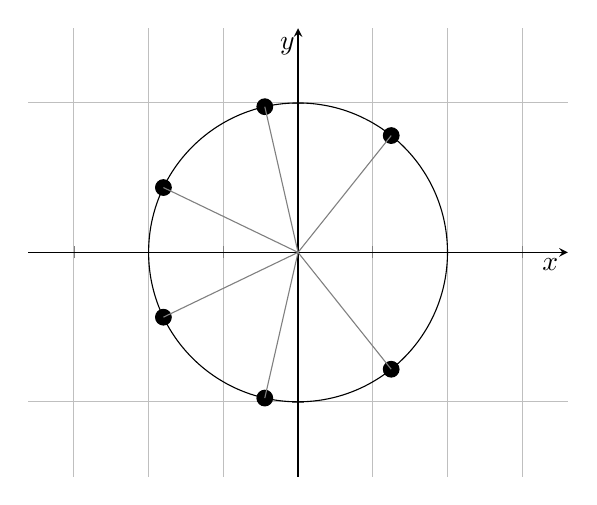
\begin{tikzpicture}
        \begin{axis}[
            grid=both, axis equal,
            ymin=-1.5, ymax=1.5,
            xmin=-1.5, xmax=1.5,
            xticklabel=\empty,yticklabel=\empty,
            axis lines = middle,
            xlabel=\(x\), ylabel=\(y\),
            label style = {at={(ticklabel cs:1,1)}}
        ]  
            \draw (axis cs:0,0) circle [black, radius=1];
            
            \pgfplotsinvokeforeach{1,2,...,6}{
                % Draw the roots of unity
                % Use \pgfplotsforeach as described in https://tex.stackexchange.com/a/170670/263993
                \node[draw, circle, inner sep=2pt, fill] at (axis cs:{cos(deg(2 * pi * #1 / 7))},{sin(deg(2 * pi * #1 /7))}) {};
                
                \draw [thin, gray] (axis cs:0,0) -- (axis cs:{cos(deg(2 * pi * #1 / 7))},{sin(deg(2 * pi * #1 /7))});
            }
        \end{axis}
    \end{tikzpicture}
    \caption*{Primitive roots of unity for \(p = 7\)}
\end{figure}
\end{frame}

\begin{frame}
\frametitle{Cyclotomic fields}

Let \(G\) denote the group
\[
    G = \Gal{\rationals\left(\zeta_p\right)}{\rationals}
\]
i.e.\ the group of field automorphisms of \(\rationals\left(\zeta_p\right)\) which act as the identity on the base field \(\rationals\).

\vspace{1em}

\begin{proposition}
\(G\) is isomorphic to \(\left(\integers/p\integers\right)^{\times}\). Each element \(\sigma_c\) is of the form \(\zeta_p \mapsto \left(\zeta_p\right)^c\) for some \(c \in \Set{1, \dots, p - 1}\).
\end{proposition}
\end{frame}

\begin{frame}
\frametitle{Mihăilescu's class number free criterion}

\begin{definition}
Let \(\integers[G]\) denote the \emph{group ring} of \(G\), i.e.\ the free \(\integers\)-module consisting of finite formal sums of the kind
\[
    \integers[G] = \Set{ \sum_{i = 1}^{k} n_i \sigma_i | n_i \in \integers, \sigma_i \in G}
\]
equipped with the multiplication induced by the group composition.
% TODO: improve explanation
\end{definition}

\vspace{1em}

We can similarly define \(\rationals[G]\), the group ring with coefficients in \(\rationals\).
\end{frame}

\begin{frame}
\frametitle{Mihăilescu's class number free criterion}

Since \(G\) acts on the field \(\rationals\left(\zeta_p\right)\), the group ring \(\integers[G]\) acts on everything defined in terms of it. \\[1em]

\(\integers[G]\) acts naturally on the group of units \(\rationals\left(\zeta_p\right)^{\times}\), the group of units of the ring of integers \(\integers\left[\zeta_p\right]^{\times}\), the group of fractional ideals, the class group etc. \\[1em]

For example, for a unit \(\alpha \in \integers\left[\zeta_p\right]^{\times}\), we have
\[
    \alpha^{\sum_{i = 1}^{k} n_i \sigma_i} = \sigma_1 (\alpha)^{n_1} \cdot \hdots \cdot \sigma_k (\alpha)^{n_k}
\]
\end{frame}

\begin{frame}
\frametitle{Stickelberger element}

\begin{definition}
The Stickelberger element is
\[
    \theta = \sum_{c = 1}^{p - 1} \left\{\frac{c}{p}\right\} \cdot \sigma_{c}^{-1} \in \rationals[G]
\]
\end{definition}
\begin{definition}
The Stickelberger ideal is
\[
    I_{S} = \integers[G] \cap \theta \, \integers[G]
\]
\end{definition}
\end{frame}

\begin{frame}
\frametitle{Stickelberger's Theorem}

\begin{theorem}[Stickelberger, 1890]
The Stickelberger ideal annihilates the class group of \(\rationals\left(\zeta_p\right)\).
\end{theorem}

\vspace{1em}

In other words, for every fractional ideal \(M\), there exists a \(\Theta \in I_S\) such that \(M^{I_S}\) is principal.
\end{frame}

\begin{frame}
\frametitle{Stickelberger's Theorem}

Stickelberger proved his theorem by looking at Gauss sums, i.e.\ sums of the form
\[
    G(\chi) = -\sum_{a \in \finitefield{p}} \chi(a) \cdot \zeta_p^{a}
\]
for \(\chi \in \finitefield{p} \to \complex^{\times}\) a character. See \cite{Washington1997} for a detailed proof.
\end{frame}

\begin{frame}
\frametitle{Mihăilescu's class number free criterion}

We have the decomposition
\[
    \frac{x^p - 1}{p (x - 1)} = \prod_{i = 1}^{p - 1} \frac{x - \zeta_p^i}{1 - \zeta_p^i}
\]
and by Cassel's relations
\[
    \frac{x^p - 1}{p (x - 1)} = u^q
\]
for some \(u \in \integers\). Hence,
\[
    \prod_{i = 1}^{p - 1} \frac{x - \zeta_p^i}{1 - \zeta_p^i} = u^q
\]
\end{frame}

\begin{frame}
\frametitle{Mihăilescu's class number free criterion}

The ideals
\[
    \beta_i = \left(\frac{x - \zeta_p^i}{1 - \zeta_p^i}\right) \integers\left[\zeta_p\right]
\]
are coprime. By the unique factorisation of ideals, they must all be \(q\) powers:
\[
    \beta_i = \symfrak{u}_i^q
\]
Mihăilescu proceeds by applying elements \(\Theta\) from the Stickelberger ideal to these ideals and performing a few calculations in the spirit of Hyyrö and Inkeri's proofs.
\end{frame}

\subsection{Primary cyclotomic units}

\begin{frame}
\frametitle{Mihăilescu's proof of the general case}

We are now ready to discuss Mihăilescu's paper \cite{Mihailescu2004} from 2004, where he finally solved Catalan's conjecture in the general case.
\end{frame}

\begin{frame}
\frametitle{Cyclotomic units and real units}

An important automorphism of the field \(\rationals\left(\zeta_p\right)\) is the one given by complex conjugation, which we will denote by \(\sigma_{-1}\). \\[1em]

The field fixed by \(\sigma_{-1}\) is called the \emph{maximal real subfield} of \(\rationals\left(\zeta_p\right)\) and will be denoted by \(\rationals\left(\zeta_p + \overline{\zeta_p}\right)\) or \(\rationals\left(\zeta_p\right)^{+}\). Its ring of integers is \(\integers\left[\zeta_p\right]^{+} = \integers\left[\zeta_p + \overline{\zeta_p}\right]\).
\end{frame}

\begin{frame}
\frametitle{Cyclotomic units and real units}

We have the following situation:
\begin{align*}
    &\begin{tikzcd}
        \rationals\left(\zeta_p\right) \\
        \rationals\left(\zeta_p + \overline{\zeta_p}\right) \arrow[u, hookrightarrow] \\
        \rationals \arrow[u, hookrightarrow]
    \end{tikzcd}
    &
    &\begin{tikzcd}
        \set{\symrm{Id}} \arrow[d, hookrightarrow] \\
        G^{+} \arrow[d, hookrightarrow] \\
        G
    \end{tikzcd}
\end{align*}
\end{frame}

\begin{frame}
\frametitle{Cyclotomic units and real units}

\begin{definition}
Let \(E\) denote the multiplicative group of \emph{real units} of \(\rationals\left(\zeta_p\right)\), i.e.\ \(E = \reals \cap \left(\rationals\left(\zeta_p\right)^{\times}\right)\).
\end{definition}

\begin{definition}
Let \(C\) be the multiplicative group generated by elements of the form
\[
    \frac{\zeta_p^k - \overline{\zeta_p^k}}{\zeta_p - \overline{\zeta_p}} \in \reals
\]
which are called \emph{cyclotomic units}.
\end{definition}
\end{frame}

\begin{frame}
\frametitle{Cyclotomic units and real units}

\begin{proposition}
\(C\) is a subgroup of \(E\) of finite index.
\end{proposition}

\vspace{1em}

This result goes back to Kummer, and it was proven using methods from analytic number theory (characters and \(L\)-functions). \\[1em]

In fact, Kummer proved an even more precise statement:
\[
    \left[E : C\right] = h_{\rationals\left(\zeta_p + \overline{\zeta_p}\right)}
\]
\end{frame}

\begin{frame}
\frametitle{Mihăilescu's proof of the general case}

\begin{definition}
An algebraic integer \(\alpha \in \integers\left[\zeta_p\right]\) is called \emph{\(q\)-primary} if there exist another \(\beta \in \integers\left[\zeta_p\right]\) such that
\[
    \alpha \equiv \beta^q \mod{(q^2) \, \integers\left[\zeta_p\right]}
\]
\end{definition}

\begin{definition}
A cyclotomic unit which is \(q\)-primary will be called a \emph{\(q\)-primary unit}. Denote the set of \(q\)-primary units by \(C_q\).
\end{definition} 

\vspace{1em}

Mihăilescu's overall proof strategy will be to focus on the relation between the subgroup \(C_q\) and \(C\).
\end{frame}

\begin{frame}
\frametitle{Mihăilescu's proof of the general case}

Mihăilescu showed that not all cyclotomic units can be \(q\)-primary if \(q \leq p\):
\begin{proposition}
If \(C_q = C\), then \(q > p\).
\end{proposition}

\vspace{1em}

Mihăilescu proved this by considering the polynomial
\[
    f(X) = \frac{(1 + X)^q - (1 + X^q)}{q X} \mod{q} \in \finitefield{q}[X]
\]
and computing how many zeros it can have in the field \(\integers\left[\zeta_p\right] / \symfrak{q}\), where \(\symfrak{q}\) is a prime ideal sitting above \(q\).
\end{frame}

\begin{frame}
\frametitle{Thaine's Theorem}

We are going to need the following result:
\begin{theorem}[Thaine, 1988]
If \(p \not\equiv 1 \mod{q}\) and \(\theta \in \integers\left[G^{+}\right]\) annihilates the \(q\)-Sylow subgroup of \(E / C\), then \(\theta\) annihilates the \(q\)-Sylow subgroup of the class group of \(\rationals\left(\zeta_p + \overline{\zeta_p}\right)\).
\end{theorem}

\vspace{1em}

Thaine's original proof \cite{Thaine1988} appeared 1988 in the Annals of Mathematics, and relies on several deep theorems from class field theory, including Chebotarev's density theorem.
\end{frame}

\begin{frame}
\frametitle{\(q\)-primary units and Catalan's equation}

Using Thaine's theorem, Mihăilescu proved the following:
\begin{figure}
    \centering
    \includegraphics[width=0.9\textwidth]{bumira-camar}
\end{figure}
where \(C^q\) is the set of \(q\)-th powers of cyclotomic units and \(\Omega \subseteq \integers[G]\) is the smallest submodule which annihilates \(C_q / C^q\). In particular, Mihăilescu proved that if \(q \notdivides p - 1\) and \(\operatorname{ann}(C_q / C^q) = \Set{ 0 }\), then \(C = C_q\).
\end{frame}

\begin{frame}
\frametitle{Bumira Camar}

Why the name for the theorem?

\begin{figure}
    \centering
    \includegraphics[width=0.9\textwidth]{bumira-camar-remark}
\end{figure}
\end{frame}

\begin{frame}
\frametitle{\(q\)-primary units and Catalan's equation}

Mihăilescu uses this theorem to link \(\Omega\) to solutions of Catalan's equation. He showed that a nontrivial solution would imply \(\Omega = \symrm{N}\) (the ideal generated by the norm element) and that all cyclotomic units would be \(q\)-primary.
\end{frame}

\begin{frame}
\frametitle{Mihăilescu's proof of Catalan's conjecture}

The final part of the proof:
\begin{theorem}
Let \(\left(x, y, p, q\right)\) be a solution to Catalan's equation for \(p\), \(q\) odd primes and suppose that \(p \not\equiv 1 \mod{q^2}\). Then \(C = C_q\).
\end{theorem}

\vspace{1em}

This theorem is proven by writing the formal power series for the ``elementary q-th root'' of an algebraic number and doing a few estimates for what its value can be, then connecting this with the ideal \(\Omega\) from before.
\end{frame}

\begin{frame}
\frametitle{What if \(p \equiv 1 \mod{q^2}\)?}

Notice that in the previous theorem we made the assumption that \(p \not\equiv 1 \mod{q^2}\) or, in other words, that \(q^2\) does \emph{not} divide \(p - 1\). \\[1em]

Mihăilescu had to manually rule out this case separately, by using estimates similar to the ones for Tijdeman's bound. Later, others gave algebraic proofs for this result.
\end{frame}

\begin{frame}
\frametitle{Mihăilescu's proof of Catalan's conjecture}

\begin{theorem}
Catalan's conjecture is true.
\end{theorem}
\begin{proof}
Suppose that \((x, y, p, q)\) is a solution to Catalan's equation with \(p\) and \(q\) odd primes and \(p \not\equiv 1 \mod{q}\). Then \(C = C_q\) by using Mihăilescu's results, but an earlier proposition shows that this must imply \(q > p\), a contradiction.
\end{proof}

\end{frame}

